\subsubsection{Analyse (Business Model)}
\subsubsection*{Domain Model}
In der Abbildung \ref{fig:domain_model_full} ist das vollständige Domain Model Model abgebildet. Um dem Leser ein klares Bild zu verschaffen, wurde dieses in die einzelnen Teilbereiche aufgeteilt.

\begin{landscape}

\begin{minipage}{\textwidth}
	\begin{figure}[H]
	\begin{center}
		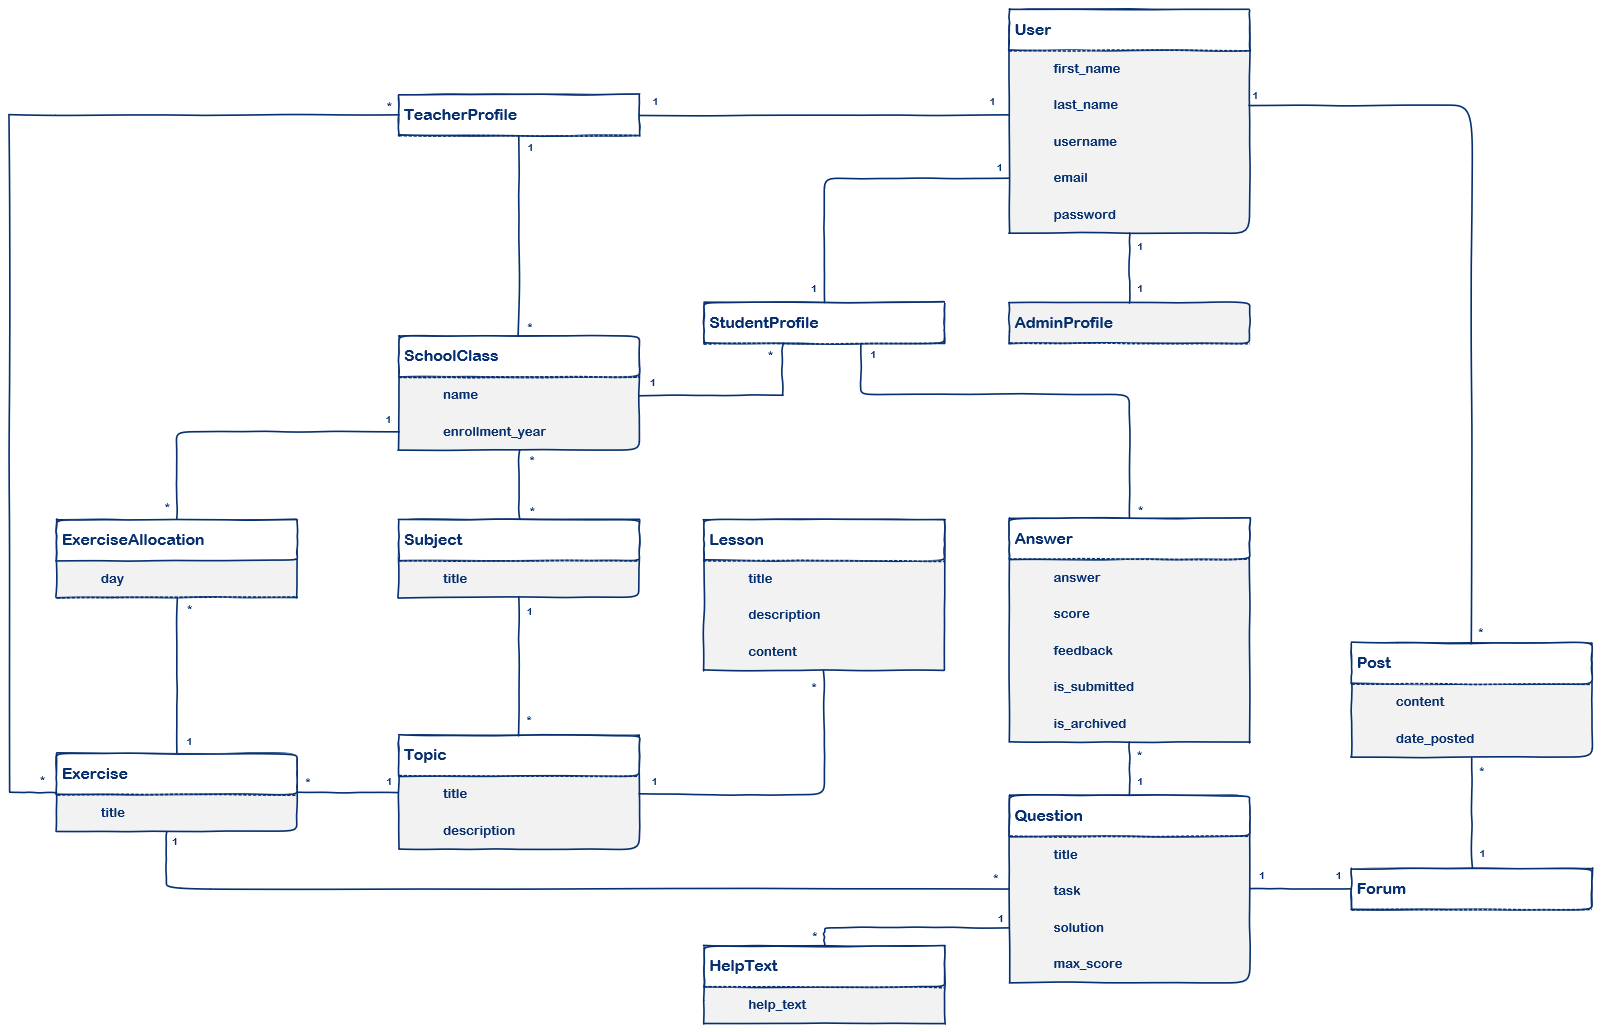
\includegraphics[width=1.4\textwidth, keepaspectratio]{images/domain_model_full.png}
  		\caption{Vollständiges Domain Model}
		\label{fig:domain_model_full}
	\end{center}
	\end{figure}
\end{minipage}

\end{landscape}

\subsubsection*{School}
Ein zentraler Punkt der Anwendung ist die Schule und das User Management. Die User sind einer der drei Rollen Student, Teacher oder Admin zugeteilt. Da jede Rolle unterschiedliche Rechte hat, konnte nicht das Standard User Model von Django selber verwendet werden. \\
Es stehen drei Möglichkeiten zur Verfügung, wie unterschiedliche User Rollen implementiert werden können.

\begin{enumerate}
	\item Unterscheidung der User anhand eines Boolean Flags
	\item Unterscheidung der User anhand eines Choices Field 
	\item Erstellung eines Profile Models mit einer 1 zu 1 Beziehung zum User Model
\end{enumerate}

Die erste Variante hat den Vorteil, dass ein User mehrere Rollen gleichzeitig haben kann. Im Gegensatz zur ersten Variante kann ein User bei der zweiten Variante nur eine Rolle annehmen kann. Diese beiden Varianten haben jedoch den Nachteil, dass jeder User die gleichen Daten hat. Möchte man einem Schüler eine Matrikelnummer zuweisen, existiert dieses Feld implizit auch für alle Lehrer und Admins. \\
Um diesem Problem aus dem Weg zu gehen, entschied man sich für die dritte Variante. Pro Rolle existiert ein Profile Model. Möchte man nur einer bestimmten Rolle ein Feld zuweisen, so kann dieses Feld im entsprechenden Profile Model hinzugefügt werden\footcite{django:user_types}. \\

\begin{figure}[H]
	\begin{center}
	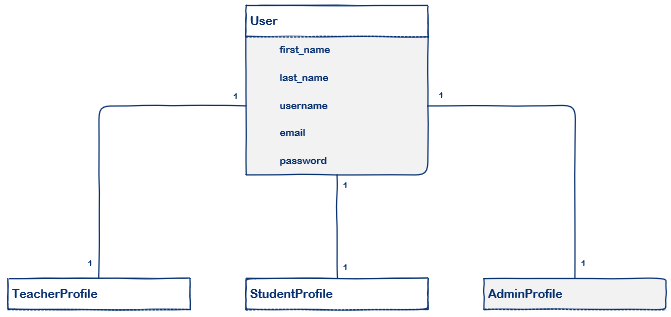
\includegraphics[width=\textwidth, keepaspectratio]{images/domain_model_user.png}
	\caption{Domain Model - User Abschnitt}
	\label{fig:domain_model_user}
	\end{center}
\end{figure}

Der Admin kann als einziger User Typ für sich alleine existieren. Schüler und Lehrer werden Klassen zugewiesen. Ein Lehrer kann gleichzeitig mehreren Klassen zugewiesen sein, ein Schüler kann sich jedoch nur in einer Klasse befinden. Für den aktuellen Stand reicht diese Funktionalität aus. Es gibt jedoch den Use Case, in welchem Schüler aus unterschiedlichen Klassen Fächer zusammen belegen. Dies ist zum Beispiel der Fall, wenn Migrationskinder aus unterschiedlichen Klassen zusammen kommen und gemeinsam ein Deutsch Nachhilfe Fach besuchen. Für diesen Fall kann man dem Student Profile ein Boolean Flag zuweisen. Falls dieses Flag gesetzt ist, hat der Schüler Zugriff auf Nachhilfe Fächer. \\

Wenn dieses Projekt als Startup weiter verfolgt wird, dann würde pro Schule eine neue Instanz der Anwendung deployed werden. So entstehen keine Multi Tenancy Probleme. Möchte man in Zukunft jedoch einen Multi Tenancy Ansatz verfolgen, müsste das Domain Model dementsprechend angepasst werden. Ein möglicher Lösungsansatz wäre, wenn jeder Schule eine eigene Subdomain, wie zum Beispiel schule-gossau.aufgaben-coach.ch, vergeben würde. Anhand der Subdomain können dann die einzelnen User identifiziert werden\footcite{django:multi_tenancy}.

\subsubsection*{Study Content}
Ein zentraler Punkt dieser Anwendung sind die Schulfächer. Pro Subject gibt es mehrere Topics. Topics wiederum können mehrere Lessons haben. \\ 

\begin{figure}[H]
\begin{center}
	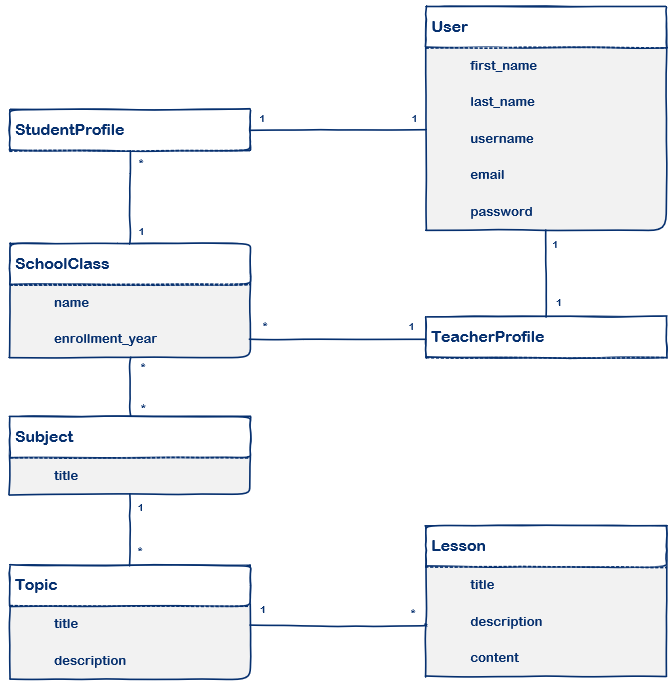
\includegraphics[width=\textwidth, keepaspectratio]{images/domain_model_study_content.png}
	\caption{Domain Model - Schulfächer}
	\label{fig:domain_model_study_content}
\end{center}
\end{figure}


Ein Subjects kann einer Klasse zugewiesen werden, welche erst dann Zugriff auf die Topics und Lessons hat. Im Moment ist es nicht möglich, einzelne Topics oder Lessons freizuschalten. Möchte man diese Funktionalität in Zukunft haben, muss eine neue Tabelle, ähnlich wie SubjectEnrollment, erstellt werden.

\subsubsection*{Exercise}
Das Herzstück der Anwendung sind die Exercises. Lehrer können Übungen erstellen, welche aus mehreren Teilaufgaben bestehen, welche wiederm mehrere Hilfestellungen haben. 

\begin{figure}[H]
\begin{center}
	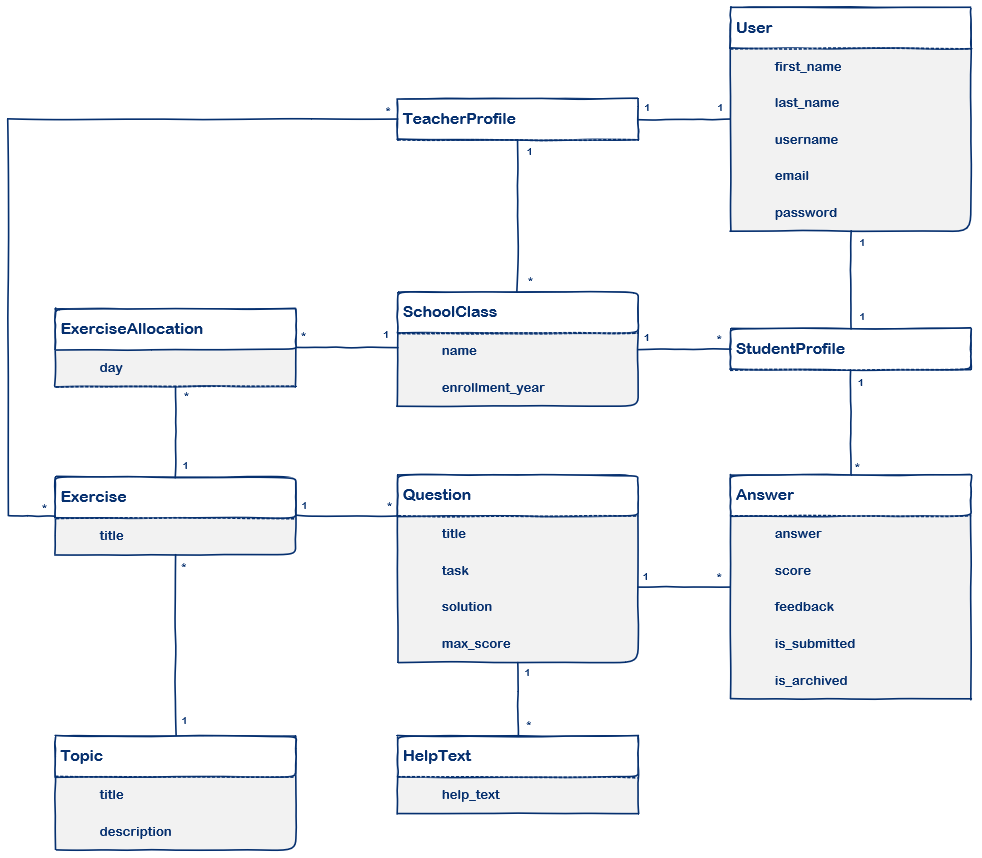
\includegraphics[width=\textwidth, keepaspectratio]{images/domain_model_exercise.png}
	\caption{Domain Model - Aufgaben}
	\label{fig:domain_model_exercise}
\end{center}
\end{figure}

Die Tabelle Answer dient zur Speicherung der Antworten von Schülern. Die beiden Felder ''is\_submitted'' und ''is\_archived'' sind für den Status der Aufgaben. Ist eine Aufgabe submitted, also abgegeben, kann sie nicht weiter vom Schüler bearbeitet werden. Erst wenn Aufgaben abgegeben sind, können sie vom Lehrer angeschaut werden. \\ 
Wurden die Aufgaben vom Lehrer korrigiert, bekommen sie den Status ''is\_archived''.

\subsubsection*{Forum}
Für jede Frage in einer Übung gibt es ein Forum. Die Schüler haben einen Ort, in welchem Fragen gestellt werden können. Da es für jede Frage ein Forum gibt, werden die Schüler auch nicht von anderen Forumsbeiträgen abgelenkt.
\begin{figure}[H]
\begin{center}
	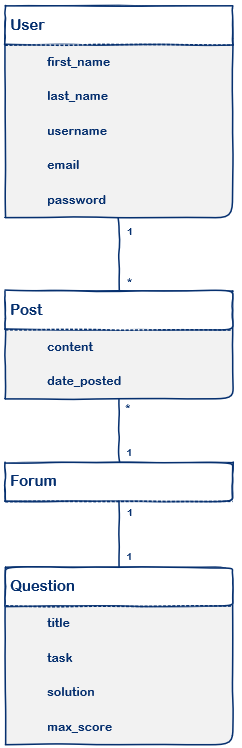
\includegraphics[width=0.3\textwidth, keepaspectratio]{images/domain_model_forum.png}
	\caption{Domain Model - Forum}
	\label{fig:domain_model_forum}
\end{center}
\end{figure}
